%************************************************
\section{The Context Client} % (fold)
\label{sec:impl_context_client}
%************************************************
The context client component needs to provide a user friendly representation of the SSM Sets, as the simulation unfolds. In Section \ref{sec:context_client} we have designed this component to work on top of the API. But, the context client also needs to represent data close to real-time. So, instead of introducing an level of indirection by connecting to the API, which in turn adds a certain delay to retrieving the response, we are using the information straight out of the SSMBundle. This means that the context client is not running on top of the API, rather it is a standalone component.\\

In the current version we have implement the context client as a web page served right out of the running simulation. Once loaded, the web page is automatically refreshed every second. A screenshot of the context client is depicted in Figure \ref{fig:impl_context_client}.
\begin{figure}[H]
	\centering
	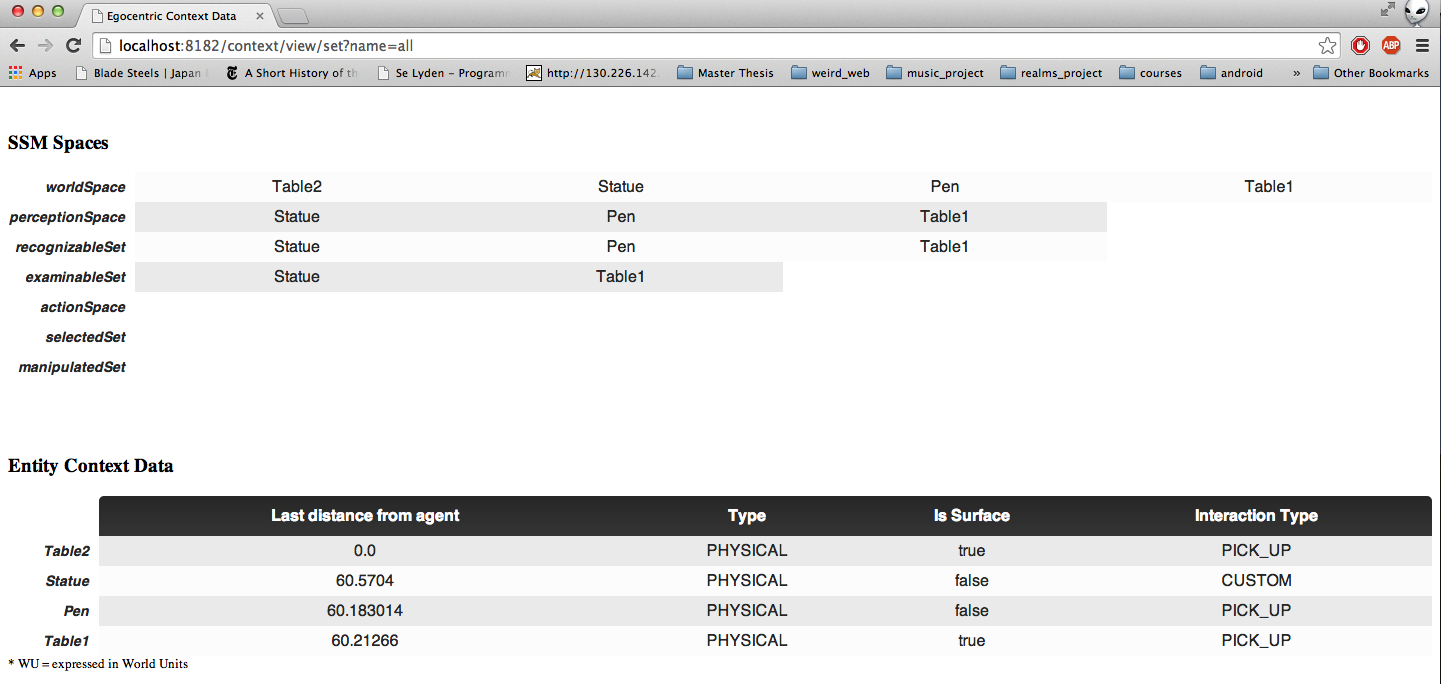
\includegraphics[width=\linewidth]{gfx/Chapter4/context_client}
	\caption{Screenshot of the Context Client}
	\label{fig:impl_context_client}
\end{figure}

To implement the context client we have used the same approach as we did with the API \ref{sec:api}. We have use the Restlet framework to create an endpoint serving HTML content. The class diagram in Figure \ref{fig:impl_context_client_class} illustrates the classes implementing this components behaviour. The ContextViewServer is initialized in the monitoring service component \ref{sec:impl_monitoring_service}. If accessed from the same computer the simulator is running on, it can be accessed on \url{http://localhost:8182/context/view}. This endpoint accepts only GET requests, each request being handled by a new instance of the ViewContextResource class.
\begin{figure}[H]
	\centering
	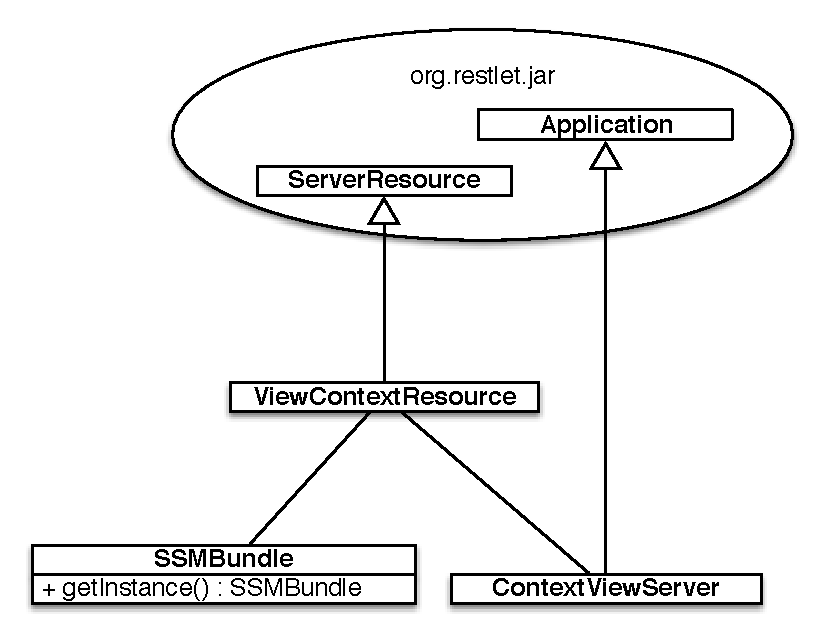
\includegraphics[width=\linewidth]{gfx/Chapter4/context_client_class}
	\caption{Class Diagram of the Context Client classes and their third party dependencies}
	\label{fig:impl_context_client_class}
\end{figure}

The endpoint accepts an URL parameter called \emph{name} to specify the name of the set the third party service wants to retrieve. The possible values are: \emph{worldSpace}, \emph{perceptionSpace}, \emph{recognizableSet}, \emph{examinableSet}, \emph{actionSpace}, \emph{selectedSet}, \emph{manipulatedSet} and \emph{all}. For example, to see the content of the World Space in the context client, the simulation user would access \url{http://localhost:8182/context/api?name=worldSpace} from a web browser.\\

The problem with the current implementation is that it does not reflect the new information immediately after a change in the context occurs. It only does so every second. To improve refresh time, we can use Web Sockets\footnote{\url{http://www.websocket.org/}} in the future work. The WebSocket specification defines a full-duplex single socket connection over which messages can be sent between client and server. This means that instead of refreshing the context client every second, the ContextViewServer could push up to date information towards the context client, whenever available, through an open web socket connection.\\

The advantage of having implemented the context client as a web page, is that no additional software installation is required. It can be accessed from any browser, on any platform.
% section impl_context_client (end)